\section {Два корня на луче}

Расположение двух корней на луче (Вариант $IV$) допускает границы четырёх типов:

\begin {enumerate} [labelindent=\parindent, leftmargin=*]
    \item {$[\alpha, +\infty)$}
    \item {$(\alpha, +\infty)$}
    \item {$(-\infty, \beta]$}
    \item {$(-\infty, \beta)$}
\end {enumerate}

Особый случай для границ типов 1 и 3 --- это попадание одного корня уравнения $f(x)=0$ в начало 
луча.

\subsection {Границы 1 типа}

Например, особому случаю 1 типа границ будет соответствовать следующая ситуация:

\begin {figure} [h]
    \begin {minipage} [t] {\linewidth}
        \centering
        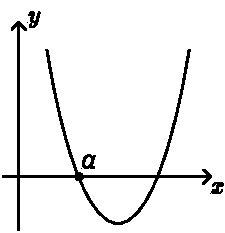
\includegraphics [width=0.3\linewidth] {image/image_10.pdf}
    \end {minipage}
\end {figure}

Чтобы обработать этот случай, необходимо рассмотреть прохождение параболы $y = f(x)$
через точку $\alpha$. То есть решить уравнение

$$ f(\alpha) = 0 $$

Подставляем полученные параметры в трёхчлен $f(x)$, и выбираем из них те, при которых второй корень 
существует и лежит на луче $[\alpha, +\infty)$. Это можно
сделать с помощью теоремы Виета или проверки соответствующих условий:
\begin {equation*}
    x_0 > \alpha
\end {equation*}

\pagebreak

\subsection {Границы 2 и 4 типов. Общий случай}

Границы 2 и 4 типов исключают особые случаи и являются, вообще говоря, общим случаем.
Например, особому случаю второго типа границ будет соответствовать следующая ситуация:

\begin {figure} [h]
    \begin {minipage} [t] {\linewidth}
        \centering
        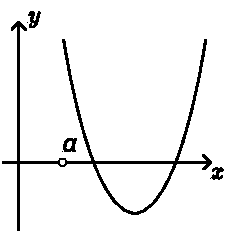
\includegraphics [width=0.3\linewidth] {image/image_11.pdf}
    \end {minipage}
\end {figure} 

Чтобы оба корня были внутри луча $[\alpha, +\infty)$, необходимо выполнение следующих условий:

\begin {itemize}
    \item {существует два корня}
    \item {вершина параболы лежит на луче}
    \item {на конце луча значение квадратного трёхчлена положительно (с точностью до умножения на
           коэффициент $a$)}
\end {itemize}

Получаем следующую систему:

\begin {equation*}
    \begin {cases}
        D > 0
        \\
        x_0 > \alpha
        \\
        a \cdot f(\alpha) > 0
    \end {cases}
\end {equation*}

Как уже говорилось, чтобы получить полное решение, нужно объединить особые случаи с общим решением
задачи. 